\chapter[Molten Salt Reactors]{Molten Salt Reactors}


\section{History}

Developing of \glspl{MSR} started in the late 1940's as part of the United States' program to design a nuclear powered airplane. Particularly  liquid fuel appeared to offer number of advantages, and experiments to demonstrate the feasibility of molten salt fuels were begun in 1947 on ``the initiative of V.P.Calkins, Kermit Anderson, and E.S.Bettis. At the enthusiastic urging of Bettis and on the recommendation of W.R.Grimes, R.C.Briant adopted molten fluoride salts in 1950 as the main line effort of the \glsfirst{ORNL}'s Aircraft Nuclear Propulsion program." The flourides appeared exceptionally suitable because they have high solubility for uranium, are among the most stable of chemical compounds, have low vapor pressure even at temperature more than 1300$^{\circ}$C, have fairly good hydraulic and thermal properties, do not react furiously with air of water, are not damaged by hight neutron fluxes, and are inert to some common structural materials \cite{rosenthal_molten-salt_1970}.

A small test reactor, the \gls{ARE}, was built at Oak Ridge site to probe the use of molten flouride fuels for aircraft propulsion reactors and to study the nuclear stability of the circulating fuel system. Fuel salt for the \gls{ARE} was a mixture of NaF, ZrF$_4$, and UF$_4$, BeO served as moderator, and all the piping was nickel-chromium alloy Inconel. The experiment was successful: in 1954 the \gls{ARE} was operated for 9 days at steady-state outlet temperatures up to 860$^{\circ}$C and at powers up to 2.5 MW$_{(th)}$. No mechanical or chemical problems were observed, and the reactor was found to be stable and self-regulating.

Great potential of \glspl{MSR} for civilian power application was recognized from the beginning of Aircraft Nuclear Propulsion program, and in 1956 H.G.MacPherson founded a group to study the technical characteristics, nuclear performance, and economics of molten salt converting and breeding reactors. After few years of research with number of concepts, MacPherson and his colleagues concluded that graphite-moderated thermal reactors operating on a thorium fuel cycle would be the best choice for applying molten salt systems for producing economic energy. Breeding $^{233}$U from $^{232}$Th was found to give better performance in a molten salt thermal reactor neutron energy spectrum than a uranium fuel cycle in which depleted uranium ($^{238}$U) is the fertile material and fissile $^{239}$Pu is produced and recycled. Homogeneous reactor designs that have entire core consist of liquid sal were rejected because the limited moderation by the salt components did not prove to make good thermal reactor comparing with one moderated by graphite. Furthermore, intermediate spectrum reactors did not appear to have high enough breeding ratios to compensate for their higher inventory of fuel. Later studies of fast spectrum molten salt reactors \cite{kasten_mosel_1964} has shown that effective breeding could be obtained with extremely high power densities that needed to avoid excessive fissile inventories. Acceptable  power densities appeared challenging to achieve without using novel and untested heat transfer technologies.

Two types of graphite-moderated reactors were selected by MacPherson's group for further research: single-fluid reactors in which thorium and uranium are dissolved in the same carrier salt, and two-fluid design in which a fertile salt accommodated $^{232}$Th is separated from the fissile salt which contains $^{233}$U and/or $^{239}$Pu as initial fissile load for reactor startup. The two-fluid reactor could operates as breeder but construction materials separating flows would significantly deteriorate neutron economy and, consequently, breeding ratio. The single-fluid design is much simplier, easier to build and offers lower power costs, even for that time technology which could only achive breeding ratio slightly below 1.0. The chemical reprocessing method namely fluoride volatility process, which separates uranium from flouride salts, had been already demonstrated during \gls{ARE} for recovery uranium from \gls{ARE} fuel salt and might be used for partial reprocessing of salts from another type of reactor.

U.S. Atomic Energy Commission task force have considered results of the \gls{ORNL} research and made a comparative evaluation of fluid-fueled reactors early in 1959. One conclusion of the task force was that the \gls{MSR} even limited in potential breeding gain, had ``the highest probability of achieving technical feasibility." \cite{noauthor_report_1959}

In 1960s more complete conceptual \gls{MSR} designs have been developed. \gls{ORNL} conculed that both single-fluid and two-fluid concepts whould lead to low-power-cost reactors, and that progressing to the breeder either directly or using the converter would create reactors with good fuel utilization characteristics \cite{rosenthal_molten-salt_1970}. Because of many of the features of commercial power reactors would differ from those for the \gls{ARE}, and the \gls{ARE} had beed operated only a short period of time, new reactor experiment with molten salt was necessary to investigate some of the technology for civilian power reactors.

The developing of the \gls{MSRE} was started in 1960. Creators selected a single-fluid design because it is similar to a converter, but the fuel salt did not contain thorium, consequently, was similar to the fuel salt composition for a two-fluid breeder. The \gls{MSRE} fuel salt is a mixture of uranium, $^7$Li, beryllium, and sirconium fluorides. Bare graphite serves as the moderator because the salt cannot penetrate into its pores if the pore sizes are small. Specially developed in the aircraft program nickel-based alloy INOR-8 (also called Hastelloy-N) for use with molten fluorides was employed as a main constuction material for piping and other elements of the system. The maximum power is about 8MW$_{th}$, and the heat is dissipated to the atmosphere \cite{haubenreich_experience_1970}.

Construction of the \gls{MSRE} has begun in 1962, and the reactor first became critical in 1965. Figure~\ref{fig:msre} has shown graphite reactor core assembling. Continuous operation at full power level began in December 1966. Successful completion of a six-month test campaign in March of 1968 closed the first phase of operation, all initial objectives were achived. The molten fluoride fuel salt was used in the reactor core for many month at temperatures $\geq$649$^{\circ}$C without corrosive damaging of the metal and graphite elements of the system. All reactor equipment worked reliably, radioactive liquids and gases were holded safely, te fuel salt was absolutely stable. Xenon was removed continuously from the salt. Radiactive components was reapaired or replaced in acceptable time without overexposing mainenance personnel.

The second stage of \gls{MSRE} has started in August 1968 when a small chemical processing facility connected with the reactor was used to remove the original uranium from the fuel salt using fluorine gas. $^{233}$U fuel was added to the same carrier salt, and on October 2 the \gls{MSRE} begun operation on $^{233}$U. Six days later the power was achieved 100 kW by Glenn T.Seaborg, Chairman of the U.S. Atomic Energy Commission, bringing to power the first in a world reactor operating on $^{233}$U \cite{haubenreich_experience_1970}.

\begin{figure}[htp!] % replace 't' with 'b' to 
  \centering
  \vspace{-0.3em}
  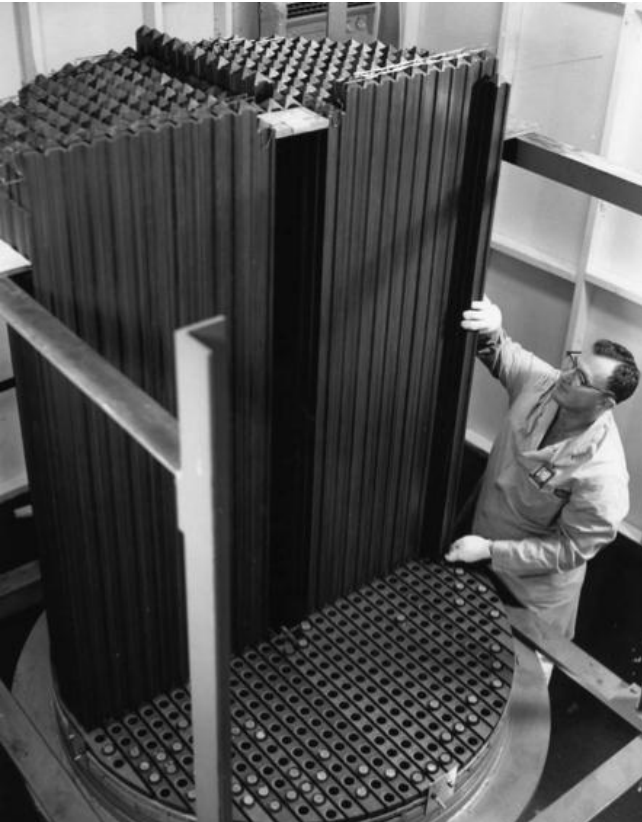
\includegraphics[width=0.75\linewidth]{msre_view.png}
  \caption{The \gls{MSRE} core, shown while being assembled, contains about 1.95 m$^3$ of reactor graphite. The 1140 fuel channels contain about 0.57m$^3$ of fuel salt.}
  \vspace{-0.6em}
  \label{fig:msre}
\end{figure}
\FloatBarrier

After \gls{MSRE} was build and brought into operation, most of the research and development work on \glspl{MSR} was in support of the \gls{MSRE}. However, molten fluoride salts chemistry keep developing during this period, i.e. was discovered method of separation lithium fluoride and beryllium fluoride from rare earths by vacuum distillation at temperature about 1000$^{\circ}$C. This method provided an inexpensive, on-site way for recovering valuable rare materials, following this, the study effort for future reactors changed focus to a two-fluid breeder. In this reactor the fuel salt should be fluorinated to recover the uranium and distilled to separate carrier salt from fission products. The blanket salt would be reprocessed by just fluorination because only few fission products might be generated in the blanket if the fissile material concentration were kept low and no fission happens in the blanket. Graphite tubes in the core were designed to prevent the fuel and fertile streams from mixing.

Two-fluid systems analysis have shown that breeding ratio could be about 1.07, which with low fissile inventory would lead to relatively good fuel utilization. Therefore, the development effort for future reactors was concentrated at the futures of two-fluid breeders. The main drawback of those reactors was identified as graphite pipes damaging by very high neutron fluxes.

Later, in 1967, new experimental information obtained from \gls{MSRE} and an advance in core design lead to change \gls{ORNL} molten salt program R\&D focus from the two-fluid to a single-fluid breeder. This switch was based on concerns about graphite behavior at higher radiation exposures that had been achieved previously, graphite changes dimensions more rapidly than had been acticipated. To use that kind of graphite in \gls{MSBR} it was necessary to lower the core power density to achieve acceptable graphite lifetime, and to plan on replacement of the core at realistically frequent intervals. Furthermore, complexities in the assembly of the core required the entire core and reactor vessel replacement when any graphite element reached its irradiation limit or developed a leak \cite{rosenthal_molten-salt_1970}.

Because of problems associated with long graphite exposure and significant development of chemical processing \gls{ORNL} decided to change focus to single-fluid breeder.To achieve acceptable breeding ratio in single-fluid reactor, $^{233}$Pa (27.4-day half-life) must be separated from the fuel salt and held up outside the core until it decays to $^{233}$U. Laboratory experiments demonstrated liquid-liquid extraction process for removing protactinium and uranium from molte fluoride salts. The method is to exchange throium and lithium dissolved in molten bismuth for the components to be removed from the salt.Additional data have confirmed that the uraniuum can be selectively separted from the salt, the protctinium can be trapped in the salt in a decay tank, and the uranium can be returned back to the fuel salt by electrolysis for the further transfer to the core. Analysis indicated that the extraction and electrolysis could be carried out rapidly and continuously.

The fertile ``blanket'' in the single-fluid breeder is obtained by increasing the volume fraction of fuel salt and reducing the volume fraction of graphite in the outer part of the reactor. This advanced core design makes the outer region undermoderated and increases neutron capture there by the thorium. Moreover, most of neutrons are born at some distance from the reactor boundary, and captures in outer region reduce the neutron leakage. Further studies indicated that the fuel utilization in single-fluid, two-region \gls{MSR} can be as good as in two-fluid prototype, and even with the limitation on graphite lifetim the economics might be better. Thus, in 1968 \gls{ORNL} \gls{MSR} Program was oriented toward the development of single-fluid breeder reactor.

Despite the success of \gls{ARE} and \gls{MSRE}, the \gls{MSR} program closed down in the early 1970s in favor of the liquid metal fast-breeder reactor (LMFBR),\cite{macpherson_molten_1985} after which research stagnated in the United States. As of 2018, the \gls{ARE} and \gls{MSRE} remained the only molten-salt reactors ever operated.

Recently, interest in \glspl{MSR} has resurged, with multiple new companies pursuing commercialization of \gls{MSR} designs\footnote{Examples include both liquid-fueled molten salt designs from Transatomic, Terrapower, Terrestrial, and Thorcon.}. China initiated a thorium molten salt reactor research project, demonstration of the liquid fuel version (TMSR-LF) are targeted for 2024. European Union funding Safety Assessment of the Molten Salt Fast Reactor (SAMOFAR), in which several European research institutes and universities developing various molten salt reactor prototypes such as \gls{MSFR}, \gls{MOSART}, \gls{FHR}.
To further develop these \gls{MSR} concepts, particularly with respect to their strategies for online reprocessing and refueling, computational analysis methods capturing their unique reactor physics and process chemistry are needed.

\section{Literature review}

While most contemporary nuclear reactor physics software is unable to perform depletion calculations in an online reprocessing regime. Furthermore, no established liquid-fueled \gls{MSR} tool for neutronics and fuel cycle evaluation, there are codes from universities, research institutions, and internally developed tools for online refueling approximation \cite{serp_molten_2014}. The foundation for these tools was based on early \gls{MSR} programs  methods at \gls{ORNL}, which integrated neutronic and fuel cycle codes \cite{bauman_rod:_1971} into operational plant tools \cite{kee_mrpp:_1976} for \gls{MSR} and reprocessing system designing. More recent research efforts in Europe and Asia mainly focused on fast spectrum reactors fuel cycle analysis and use some external tools to couple neutron transport and depletion codes to take into account continuous feeds and removals in \glspl{MSR}. Four of these works listed in table~\ref{tab:fs_codes}.

\begin{table}[h!]
\centering
\caption{Methods for fast spectrum system fuel cycle analysis.}
\begin{tabular}{ |m{0.02\textwidth}|m{0.2\textwidth}|m{0.2\textwidth}|m{0.45\textwidth}|} 
\hline
\# & Neutronic code  & Depletion code    & Authors         \\[5pt]
\hline
1 & \gls{MCNP}      & REM  & Nuttin \emph{et al.}, 2005; Doligez \emph{et al.}, 2014; Heuer \emph{et al.}, 2014      \\[5pt]
\hline
2 & ERANOS      & ERANOS     & Fiorina \emph{et al.}, 2013 \\[5pt]
\hline
3 & KENO-IV     & ORIGEN     & Sheu \emph{et al.}, 2013 \\[5pt]
\hline
4 & SERPENT 2   & SERPENT 2  & Aufiero \emph{et al.}, 2013 \\[5pt]
\hline
\end{tabular}
  \label{tab:fs_codes}
\end{table}

Most of these methods are applicable to thermal spectrum reactors, moreover, additional tools developed specifically for thermal \gls{MSR} applications listed in table~\ref{tab:th_codes}.

\begin{table}[h!]
\centering
\caption{Tools and approaches for thermal spectrum system fuel cycle analysis.}
\begin{tabular}{ |m{0.02\textwidth}|m{0.2\textwidth}|m{0.2\textwidth}|m{0.45\textwidth}|} 
\hline
\# & Neutronic code  & Depletion code    & Authors         \\[5pt]
\hline
5 & MCODE      & ORIGEN2      & Ahmad \emph{et al.}, 2015      \\[5pt]
\hline
6 & \gls{MCNP}      & CINDER90     & Park \emph{et al.}, 2015; Jeong \emph{et al.}, 2016 \\[5pt]
\hline
7 & SCALE      & SCALE/ ChemTriton     & Powers \emph{et al.}, 2014; Brown \emph{et al.}, 2015; Gehin and Powers, 2016; Betzler \emph{et al.}, 2017 \\[5pt]
\hline
8 & SERPENT 2      & SERPENT 2     & Rykhlevskii \emph{et al.}, 2017 \\[5pt]
\hline
\end{tabular}
  \label{tab:th_codes}
\end{table}

Methods (1,3,4) provide some form of reactivity control, and methods (1,4,5,6,8) use inventory of all nuclides in depletion calculations. In addition, approaches (1,4,8) provide opportunity to work with true continuous feeds and removals. Moreover, most of these efforts except (6) considered only simplified unit-cell geometry because depletion computations for few year cycle are very computationally expesive even for simple models. The unit-cell models may produce reliable results for homogeneous reactor cores (i.e. \gls{MSFR}, \gls{MOSART}) or for one-region single-fluid reactor design (i.e. \gls{MSRE}). Two-region \gls{MSBR} must be simulated using whole-core model to represent different neutron transport in inner and outer region of the core.

Current study most similar to the works described in (3,6,7), including developing new external open-source tool for online reprocessing simulation Saltproc which works with Monte Carlo code SERPENT 2. 

Powers \emph{et al.} suggested a novel method for conducting 
depletion simulations for \gls{MSR}. This suggested method takes into account 
fuel salt composition changes due to online reprocessing and refueling based on the deterministic computer code NEWT in SCALE \cite{powers_new_2013}. This approach was later used by Jeong \emph{et al.} to find an equilibrium fuel composition for the \gls{MSBR} and was validated with a \gls{MCNP}/CINDER90 model \cite{jeong_equilibrium_2016}. 

The key advantages of \gls{MSR}s generally pertain to improved fuel utilization
and reactor safety. In contrast to legacy reactors, only moderator fast neutron
damage and fuel chemistry evolution limit burnup. A clever configuration of moderator
as in \cite{engel_conceptual_1980} can enable reactor operation without opening the vessel
for thirty or more years. Further, several fission products selectively precipitate onto
nickel surfaces in fluoride salt, as documented in \cite{engel_conceptual_1980}, thus reducing
unwanted neutron absorption. Lastly, the epithermal spectrum of graphite-moderated salt reactors
incinerates plutonium more efficiently, thus reducing long-lived transuranic waste production \cite{engel_conceptual_1980}.
The sum of these characteristics implies the \gls{MSR} uniqely ameliorates spent fuel burden whilst
extending nuclear fuel resources. To top all these benefits off, xenon transients become moot in
\gls{MSR}s due to its insolubility in salt, thus narrowing transient analysis focus to thermalhydraulic
concerns.

Simulation tools developed by many authors successfully describe steady-state and
transient behavior of myriad \gls{MSR} concepts. Krepel et al. extended the in-house \gls{LWR}
diffusion code DYN3D to consider drift of delayed neutron precursors alongside
the reactor temperature profile, re-casting the extended code as
DYN3D-MSR \cite{krepel_dyn3d-msr_2007}. That work compared DYN3D-MSR against
experimental \gls{MSRE} data and then used it to simulate local fuel channel
blockages as well as local temperature perturbations.